% Created 2021-05-09 Sun 21:43
% Intended LaTeX compiler: pdflatex
\documentclass[11pt]{article}
\usepackage[utf8]{inputenc}
\usepackage[T1]{fontenc}
\usepackage{graphicx}
\usepackage{grffile}
\usepackage{longtable}
\usepackage{wrapfig}
\usepackage{rotating}
\usepackage[normalem]{ulem}
\usepackage{amsmath}
\usepackage{textcomp}
\usepackage{amssymb}
\usepackage{capt-of}
\usepackage{hyperref}
\usepackage[spanish]{babel}
\usepackage[margin=1.5cm]{geometry}
\usepackage{arev}
\usepackage{minted}
\author{Edgar Quiroz}
\date{\today}
\title{Serpientes y Escaleras a distancia\\\medskip
\large Versión de sólo texto para Google Meet}
\hypersetup{
 pdfauthor={Edgar Quiroz},
 pdftitle={Serpientes y Escaleras a distancia},
 pdfkeywords={},
 pdfsubject={},
 pdfcreator={Emacs 27.2 (Org mode 9.5)}, 
 pdflang={Spanish}}
\begin{document}

\maketitle

\section{Planteamiento}
\label{sec:org35bb3ac}

Diseñar un pequeño \texttt{CLI} para el juego de serpientes y escaleras planteado
anteriormente.

\subsection{Diagramas de clases}
\label{sec:org4c3e3a8}

\begin{figure}[htbp]
\centering
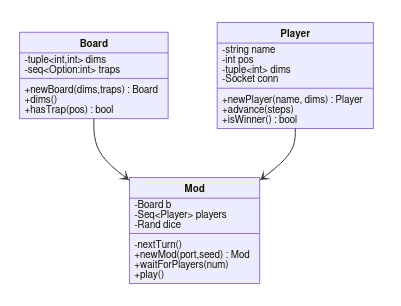
\includegraphics[scale=0.75]{imgs/mod_class.png}
\caption{\label{fig:mod-class}Clases para el moderador}
\end{figure}

\begin{figure}[htbp]
\centering
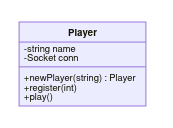
\includegraphics[scale=0.75]{imgs/player_class.png}
\caption{\label{fig:player-class}Clases para el jugador}
\end{figure}


\section{Correr}
\label{sec:orgc5fe24e}

\begin{minted}[]{bash}
nimble build
\end{minted}

Que crea dos ejecutables. \texttt{snlMod} es el programa que para el moderador que
levante el servidor para jugar. \texttt{snlPlay} es el programa para los jugadore que
se conectarán al servidor del moderador.

\section{Pruebas}
\label{sec:orgcb6e6b6}

\begin{minted}[]{bash}
nimble test
\end{minted}

Las pruebas están hechas con el paquete \texttt{unittest}. De momento no hay pruebas
para los sockets.
\end{document}
